\documentclass[a4paper, 12pt]{article}
\usepackage[utf8]{inputenc}
\usepackage[american]{babel}
\usepackage[margin=1in]{geometry}
\usepackage{mathtools}
\usepackage{fancyhdr}
\usepackage{tikz}
\usetikzlibrary{shapes, calc}
\setlength{\headheight}{15.2pt}
\pagestyle{fancy}
\lhead[]{Joseph Petitti}
\rhead[]{Homework 2}
\chead[]{Database Systems II}

\begin{document}

\section*{Problem 1}

\subsection*{(a) LRU Replacement Policy}

\begin{table}[h]
	\centering
	\begin{tabular}{l c c c c c c c c c c c c c c c}
		Instruction: & 1* & 2* & 3* & \underline{1} & 4* & 5* & \underline{3} &
		\underline{4} & 1 & 6 & 7 & 8* & 9* & 5 & 10 \\
		\hline
		Frame 1 & \textbf{1} & \textbf{1} & \textbf{1} & 1 & 1 & 1 & 1 & 1 & 1 &
		1 & 1 & 1 & 1 & 1 & 10 \\
		Frame 2 & & \textbf{2} & \textbf{2} & \textbf{2} & \textbf{2} &
		\textbf{2} & \textbf{2} & \textbf{2} & \textbf{2} & \textbf{2} &
		\textbf{2} & \textbf{2} & \textbf{2} & \textbf{2} & \textbf{2} \\
		Frame 3 & & & \textbf{3} & \textbf{3} & \textbf{3} & \textbf{3} & 3 & 3
		& 3 & 3 & 3 & \textbf{8} & \textbf{8} & \textbf{8} & \textbf{8} \\
		Frame 4 & & & & & \textbf{4} & \textbf{4} & \textbf{4} & 4 & 4 & 4 & 4 &
		4 & \textbf{9} & \textbf{9} & \textbf{9} \\
		Frame 5 & & & & & & \textbf{5} & \textbf{5} & \textbf{5} & \textbf{5} &
		\textbf{5} & \textbf{5} & \textbf{5} & \textbf{5} & \textbf{5} &
		\textbf{5} \\
		Frame 6 & & & & & & & & & & 6 & 6 & 6 & 6 & 6 & 6 \\
		Frame 7 & & & & & & & & & & & 7 & 7 & 7 & 7 & 7 \\
	\end{tabular}
\end{table}

Note: pages in bold are pinned.

\subsection*{(b) Clock Replacement Policy}

Note: a subscrpt \textit{p} indicates that a page is pinned, and a subscript
\textit{r} indicates that the reference bit is set to 1.

{
\centering

\subsubsection*{1*}
\begin{tikzpicture}
	\def \n {7}
	\def \radius {3cm}
	
	\node[] (maintopic) at (0:0) {};
	
	\node[draw, rectangle] (first)   at ({360/\n * 0 + 90}:\radius)
		{$1_{pr}$};
	\node[draw, rectangle] (second)  at ({360/\n * 6 + 90}:\radius) 
		{ };
	\node[draw, rectangle] (third)   at ({360/\n * 5 + 90}:\radius) 
		{ };
	\node[draw, rectangle] (fourth)  at ({360/\n * 4 + 90}:\radius) 
		{ };
	\node[draw, rectangle] (fifth)   at ({360/\n * 3 + 90}:\radius) 
		{ };
	\node[draw, rectangle] (sixth)   at ({360/\n * 2 + 90}:\radius) 
		{ };
	\node[draw, rectangle] (seventh) at ({360/\n * 1 + 90}:\radius) 
		{ };

	\draw[->, very thick, >=latex] (maintopic) -- (second);
\end{tikzpicture}

\subsubsection*{2*}
\begin{tikzpicture}
	\def \n {7}
	\def \radius {3cm}
	
	\node[] (maintopic) at (0:0) {};
	
	\node[draw, rectangle] (first)   at ({360/\n * 0 + 90}:\radius)
		{$1_{pr}$};
		{\textbf{\textit{1}}};
	\node[draw, rectangle] (second)  at ({360/\n * 6 + 90}:\radius) 
		{$2_{pr}$};
		{\textbf{\textit{2}}};
	\node[draw, rectangle] (third)   at ({360/\n * 5 + 90}:\radius) 
		{ };
	\node[draw, rectangle] (fourth)  at ({360/\n * 4 + 90}:\radius) 
		{ };
	\node[draw, rectangle] (fifth)   at ({360/\n * 3 + 90}:\radius) 
		{ };
	\node[draw, rectangle] (sixth)   at ({360/\n * 2 + 90}:\radius) 
		{ };
	\node[draw, rectangle] (seventh) at ({360/\n * 1 + 90}:\radius) 
		{ };

	\draw[->, very thick, >=latex] (maintopic) -- (third);
\end{tikzpicture}

\subsubsection*{3*}
\begin{tikzpicture}
	\def \n {7}
	\def \radius {3cm}
	
	\node[] (maintopic) at (0:0) {};
	
	\node[draw, rectangle] (first)   at ({360/\n * 0 + 90}:\radius)
		{$1_{pr}$};
	\node[draw, rectangle] (second)  at ({360/\n * 6 + 90}:\radius) 
		{$2_{pr}$};
	\node[draw, rectangle] (third)   at ({360/\n * 5 + 90}:\radius) 
		{$3_{pr}$};
	\node[draw, rectangle] (fourth)  at ({360/\n * 4 + 90}:\radius) 
		{ };
	\node[draw, rectangle] (fifth)   at ({360/\n * 3 + 90}:\radius) 
		{ };
	\node[draw, rectangle] (sixth)   at ({360/\n * 2 + 90}:\radius) 
		{ };
	\node[draw, rectangle] (seventh) at ({360/\n * 1 + 90}:\radius) 
		{ };

	\draw[->, very thick, >=latex] (maintopic) -- (fourth);
\end{tikzpicture}

\subsubsection*{\underline{1}}
\begin{tikzpicture}
	\def \n {7}
	\def \radius {3cm}
	
	\node[] (maintopic) at (0:0) {};
	
	\node[draw, rectangle] (first)   at ({360/\n * 0 + 90}:\radius)
		{$1_{r}$};
	\node[draw, rectangle] (second)  at ({360/\n * 6 + 90}:\radius) 
		{$2_{pr}$};
	\node[draw, rectangle] (third)   at ({360/\n * 5 + 90}:\radius) 
		{$3_{pr}$};
	\node[draw, rectangle] (fourth)  at ({360/\n * 4 + 90}:\radius) 
		{ };
	\node[draw, rectangle] (fifth)   at ({360/\n * 3 + 90}:\radius) 
		{ };
	\node[draw, rectangle] (sixth)   at ({360/\n * 2 + 90}:\radius) 
		{ };
	\node[draw, rectangle] (seventh) at ({360/\n * 1 + 90}:\radius) 
		{ };

	\draw[->, very thick, >=latex] (maintopic) -- (fourth);
\end{tikzpicture}

\subsubsection*{4*}
\begin{tikzpicture}
	\def \n {7}
	\def \radius {3cm}
	
	\node[] (maintopic) at (0:0) {};
	
	\node[draw, rectangle] (first)   at ({360/\n * 0 + 90}:\radius)
		{$1_{r}$};
	\node[draw, rectangle] (second)  at ({360/\n * 6 + 90}:\radius) 
		{$2_{pr}$};
	\node[draw, rectangle] (third)   at ({360/\n * 5 + 90}:\radius) 
		{$3_{pr}$};
	\node[draw, rectangle] (fourth)  at ({360/\n * 4 + 90}:\radius) 
		{$4_{pr}$};
	\node[draw, rectangle] (fifth)   at ({360/\n * 3 + 90}:\radius) 
		{ };
	\node[draw, rectangle] (sixth)   at ({360/\n * 2 + 90}:\radius) 
		{ };
	\node[draw, rectangle] (seventh) at ({360/\n * 1 + 90}:\radius) 
		{ };

	\draw[->, very thick, >=latex] (maintopic) -- (fifth);
\end{tikzpicture}

\subsubsection*{5*}
\begin{tikzpicture}
	\def \n {7}
	\def \radius {3cm}
	
	\node[] (maintopic) at (0:0) {};
	
	\node[draw, rectangle] (first)   at ({360/\n * 0 + 90}:\radius)
		{$1_{r}$};
	\node[draw, rectangle] (second)  at ({360/\n * 6 + 90}:\radius) 
		{$2_{pr}$};
	\node[draw, rectangle] (third)   at ({360/\n * 5 + 90}:\radius) 
		{$3_{pr}$};
	\node[draw, rectangle] (fourth)  at ({360/\n * 4 + 90}:\radius) 
		{$4_{pr}$};
	\node[draw, rectangle] (fifth)   at ({360/\n * 3 + 90}:\radius) 
		{$5_{pr}$};
	\node[draw, rectangle] (sixth)   at ({360/\n * 2 + 90}:\radius) 
		{ };
	\node[draw, rectangle] (seventh) at ({360/\n * 1 + 90}:\radius) 
		{ };

	\draw[->, very thick, >=latex] (maintopic) -- (sixth);
\end{tikzpicture}

\subsubsection*{\underline{3}}
\begin{tikzpicture}
	\def \n {7}
	\def \radius {3cm}
	
	\node[] (maintopic) at (0:0) {};
	
	\node[draw, rectangle] (first)   at ({360/\n * 0 + 90}:\radius)
		{$1_{r}$};
	\node[draw, rectangle] (second)  at ({360/\n * 6 + 90}:\radius) 
		{$2_{pr}$};
	\node[draw, rectangle] (third)   at ({360/\n * 5 + 90}:\radius) 
		{$3_{r}$};
	\node[draw, rectangle] (fourth)  at ({360/\n * 4 + 90}:\radius) 
		{$4_{pr}$};
	\node[draw, rectangle] (fifth)   at ({360/\n * 3 + 90}:\radius) 
		{$5_{pr}$};
	\node[draw, rectangle] (sixth)   at ({360/\n * 2 + 90}:\radius) 
		{ };
	\node[draw, rectangle] (seventh) at ({360/\n * 1 + 90}:\radius) 
		{ };

	\draw[->, very thick, >=latex] (maintopic) -- (sixth);
\end{tikzpicture}

\subsubsection*{\underline{4}}
\begin{tikzpicture}
	\def \n {7}
	\def \radius {3cm}
	
	\node[] (maintopic) at (0:0) {};
	
	\node[draw, rectangle] (first)   at ({360/\n * 0 + 90}:\radius)
		{$1_{r}$};
	\node[draw, rectangle] (second)  at ({360/\n * 6 + 90}:\radius) 
		{$2_{pr}$};
	\node[draw, rectangle] (third)   at ({360/\n * 5 + 90}:\radius) 
		{$3_{r}$};
	\node[draw, rectangle] (fourth)  at ({360/\n * 4 + 90}:\radius) 
		{$4_{r}$};
	\node[draw, rectangle] (fifth)   at ({360/\n * 3 + 90}:\radius) 
		{$5_{pr}$};
	\node[draw, rectangle] (sixth)   at ({360/\n * 2 + 90}:\radius) 
		{ };
	\node[draw, rectangle] (seventh) at ({360/\n * 1 + 90}:\radius) 
		{ };

	\draw[->, very thick, >=latex] (maintopic) -- (sixth);
\end{tikzpicture}

\subsubsection*{1}
\begin{tikzpicture}
	\def \n {7}
	\def \radius {3cm}
	
	\node[] (maintopic) at (0:0) {};
	
	\node[draw, rectangle] (first)   at ({360/\n * 0 + 90}:\radius)
		{$1_{r}$};
	\node[draw, rectangle] (second)  at ({360/\n * 6 + 90}:\radius) 
		{$2_{pr}$};
	\node[draw, rectangle] (third)   at ({360/\n * 5 + 90}:\radius) 
		{$3_{r}$};
	\node[draw, rectangle] (fourth)  at ({360/\n * 4 + 90}:\radius) 
		{$4_{r}$};
	\node[draw, rectangle] (fifth)   at ({360/\n * 3 + 90}:\radius) 
		{$5_{pr}$};
	\node[draw, rectangle] (sixth)   at ({360/\n * 2 + 90}:\radius) 
		{ };
	\node[draw, rectangle] (seventh) at ({360/\n * 1 + 90}:\radius) 
		{ };

	\draw[->, very thick, >=latex] (maintopic) -- (sixth);
\end{tikzpicture}

\subsubsection*{6}
\begin{tikzpicture}
	\def \n {7}
	\def \radius {3cm}
	
	\node[] (maintopic) at (0:0) {};
	
	\node[draw, rectangle] (first)   at ({360/\n * 0 + 90}:\radius)
		{$1_{r}$};
	\node[draw, rectangle] (second)  at ({360/\n * 6 + 90}:\radius) 
		{$2_{pr}$};
	\node[draw, rectangle] (third)   at ({360/\n * 5 + 90}:\radius) 
		{$3_{r}$};
	\node[draw, rectangle] (fourth)  at ({360/\n * 4 + 90}:\radius) 
		{$4_{r}$};
	\node[draw, rectangle] (fifth)   at ({360/\n * 3 + 90}:\radius) 
		{$5_{pr}$};
	\node[draw, rectangle] (sixth)   at ({360/\n * 2 + 90}:\radius) 
		{$6_{r}$};
	\node[draw, rectangle] (seventh) at ({360/\n * 1 + 90}:\radius) 
		{ };

	\draw[->, very thick, >=latex] (maintopic) -- (seventh);
\end{tikzpicture}

\subsubsection*{7}
\begin{tikzpicture}
	\def \n {7}
	\def \radius {3cm}
	
	\node[] (maintopic) at (0:0) {};
	
	\node[draw, rectangle] (first)   at ({360/\n * 0 + 90}:\radius)
		{$1_{r}$};
	\node[draw, rectangle] (second)  at ({360/\n * 6 + 90}:\radius) 
		{$2_{pr}$};
	\node[draw, rectangle] (third)   at ({360/\n * 5 + 90}:\radius) 
		{$3_{r}$};
	\node[draw, rectangle] (fourth)  at ({360/\n * 4 + 90}:\radius) 
		{$4_{r}$};
	\node[draw, rectangle] (fifth)   at ({360/\n * 3 + 90}:\radius) 
		{$5_{pr}$};
	\node[draw, rectangle] (sixth)   at ({360/\n * 2 + 90}:\radius) 
		{$6_{r}$};
	\node[draw, rectangle] (seventh) at ({360/\n * 1 + 90}:\radius) 
		{$7_{r}$};

	\draw[->, very thick, >=latex] (maintopic) -- (first);
\end{tikzpicture}

\subsubsection*{8*}
\begin{tikzpicture}
	\def \n {7}
	\def \radius {3cm}
	
	\node[] (maintopic) at (0:0) {};
	
	\node[draw, rectangle] (first)   at ({360/\n * 0 + 90}:\radius)
		{$8_{pr}$};
	\node[draw, rectangle] (second)  at ({360/\n * 6 + 90}:\radius) 
		{$2_{pr}$};
	\node[draw, rectangle] (third)   at ({360/\n * 5 + 90}:\radius) 
		{$3$};
	\node[draw, rectangle] (fourth)  at ({360/\n * 4 + 90}:\radius) 
		{$4$};
	\node[draw, rectangle] (fifth)   at ({360/\n * 3 + 90}:\radius) 
		{$5_{pr}$};
	\node[draw, rectangle] (sixth)   at ({360/\n * 2 + 90}:\radius) 
		{$6$};
	\node[draw, rectangle] (seventh) at ({360/\n * 1 + 90}:\radius) 
		{$7$};

	\draw[->, very thick, >=latex] (maintopic) -- (second);
\end{tikzpicture}

\subsubsection*{9*}
\begin{tikzpicture}
	\def \n {7}
	\def \radius {3cm}
	
	\node[] (maintopic) at (0:0) {};
	
	\node[draw, rectangle] (first)   at ({360/\n * 0 + 90}:\radius)
		{$8_{pr}$};
	\node[draw, rectangle] (second)  at ({360/\n * 6 + 90}:\radius) 
		{$2_{pr}$};
	\node[draw, rectangle] (third)   at ({360/\n * 5 + 90}:\radius) 
		{$9_{pr}$};
	\node[draw, rectangle] (fourth)  at ({360/\n * 4 + 90}:\radius) 
		{$4$};
	\node[draw, rectangle] (fifth)   at ({360/\n * 3 + 90}:\radius) 
		{$5_{pr}$};
	\node[draw, rectangle] (sixth)   at ({360/\n * 2 + 90}:\radius) 
		{$6$};
	\node[draw, rectangle] (seventh) at ({360/\n * 1 + 90}:\radius) 
		{$7$};

	\draw[->, very thick, >=latex] (maintopic) -- (fourth);
\end{tikzpicture}

\subsubsection*{5}
\begin{tikzpicture}
	\def \n {7}
	\def \radius {3cm}
	
	\node[] (maintopic) at (0:0) {};
	
	\node[draw, rectangle] (first)   at ({360/\n * 0 + 90}:\radius)
		{$8_{pr}$};
	\node[draw, rectangle] (second)  at ({360/\n * 6 + 90}:\radius) 
		{$2_{pr}$};
	\node[draw, rectangle] (third)   at ({360/\n * 5 + 90}:\radius) 
		{$9_{pr}$};
	\node[draw, rectangle] (fourth)  at ({360/\n * 4 + 90}:\radius) 
		{$4$};
	\node[draw, rectangle] (fifth)   at ({360/\n * 3 + 90}:\radius) 
		{$5_{pr}$};
	\node[draw, rectangle] (sixth)   at ({360/\n * 2 + 90}:\radius) 
		{$6$};
	\node[draw, rectangle] (seventh) at ({360/\n * 1 + 90}:\radius) 
		{$7$};

	\draw[->, very thick, >=latex] (maintopic) -- (fourth);
\end{tikzpicture}

\subsubsection*{10}
\begin{tikzpicture}
	\def \n {7}
	\def \radius {3cm}
	
	\node[] (maintopic) at (0:0) {};
	
	\node[draw, rectangle] (first)   at ({360/\n * 0 + 90}:\radius)
		{$8_{pr}$};
	\node[draw, rectangle] (second)  at ({360/\n * 6 + 90}:\radius) 
		{$2_{pr}$};
	\node[draw, rectangle] (third)   at ({360/\n * 5 + 90}:\radius) 
		{$9_{pr}$};
	\node[draw, rectangle] (fourth)  at ({360/\n * 4 + 90}:\radius) 
		{$10_{r}$};
	\node[draw, rectangle] (fifth)   at ({360/\n * 3 + 90}:\radius) 
		{$5_{pr}$};
	\node[draw, rectangle] (sixth)   at ({360/\n * 2 + 90}:\radius) 
		{$6$};
	\node[draw, rectangle] (seventh) at ({360/\n * 1 + 90}:\radius) 
		{$7$};

	\draw[->, very thick, >=latex] (maintopic) -- (fifth);
\end{tikzpicture}

}

\section*{Problem 2}

\begin{enumerate}
	\item Yes. Each entry in the index would contain the value of K1 (20 bytes)
			and a pointer to the corresponding record (8 bytes). The entire data
			file contains 20 million records, so the index file would contain 20
			million records, with each record being 28 bytes. Each block can
			contain $\lfloor 8,192 / 28 \rfloor = 292$ index records. The entire
			index would therefore be $\lceil 20,000,000 / 292 \rceil = 68,494$
			blocks.
	\item Yes. Each entry in the index would contain a pointer to the start of a
			block in the data file, and the value of K1 for the first record in
			that block. Since each block in the data file contains 20 records,
			you would need $1,000,000 / 20 = 50,000$ entries in the index, which
			would take up $\lceil 50,000 / 292 \rceil = 172$ blocks.
	\item Yes. Each entry in the index would contain the value of K2 (20 bytes)
			and a pointer to the corresponding record (8 bytes). The entire data
			file contains 20 million records, so the index file would be 28
			million bytes. Each block can contain $\lfloor 8,192 / 28 \rfloor =
			292$ index records. The entire index would therefore be $\lceil
			28,000,000 / 292 \rceil = 95,891$ blocks.
	\item No. You can't build a sparse index on an unsorted file, and since R is
			only sorted on K1 a sparse index on K2 would not work (unless R
			happens to also be sorted over K2, or if you sort the file over K2
			first).
	\item Yes. You can have a second-level sparse index on the index from (1).
			Each entry in the second-level index would contain a pointer to a
			block in the dense first-level index, and the value of the first key
			K1 in that block. Because the dense first-level index would contain
			68,494 blocks, the second-level index would have to contain 68,494
			entries, each 28 bytes long. This second-level index would take up
			$\lceil 68,494 / 292 \rceil = 235$ blocks. Combined with the size of
			the first-level index it would be $68,494 + 235 = 68,729$
			blocks.
	\item Yes. You can have a second-level sparse index on the index from (2).
			Each entry in the second-level index would contain a pointer to a
			block in the sparse first-level index, and the value of the first
			key K1 in that block. Because the sparse first-level index would
			contain 172 blocks, the second-level index would have to contain 172
			entries. This is small enough to fit in a single block. Combined
			with the size of the first level index, the total size would be $172
			+ 1 = 173$ blocks.
\end{enumerate}

\section*{Problem 3}

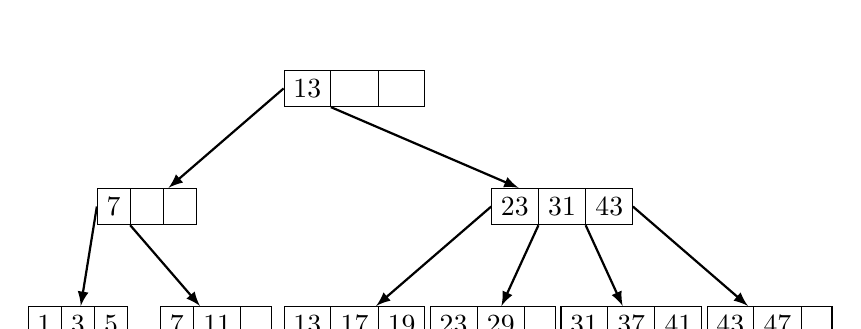
\begin{tikzpicture}
	\tikzstyle{bplus}=[rectangle split, rectangle split horizontal, rectangle
		split parts=3, draw]
	\tikzstyle{edge from parent}=[draw=none]
	\tikzstyle{every node}=[bplus]
	\tikzstyle{level 1}=[sibling distance=15em]
	\tikzstyle{level 2}=[sibling distance=5em]
	
	\node[bplus] (root) {
		\nodepart{one} 13
		\nodepart{two} \hphantom{13}
		\nodepart{three} \hphantom{13}
	}
	child {
		node (lv2a) {
			\nodepart{one} 7
			\nodepart{two} \hphantom{7}
			\nodepart{three} \hphantom{7}
		}
		child {node (leafa) {1 \nodepart{two} 3 \nodepart{three} 5}}
		child {node (leafb) {7 \nodepart{two} 11 \nodepart{three} }}
	}
	child {
		node (lv2b) {
			\nodepart{one} 23
			\nodepart{two} 31
			\nodepart{three} 43
		}
		child {node (leafc) {13 \nodepart{two} 17 \nodepart{three} 19}}
		child {node (leafd) {23 \nodepart{two} 29 \nodepart{three} }}
		child {node (leafe) {31 \nodepart{two} 37 \nodepart{three} 41}}
		child {node (leaff) {43 \nodepart{two} 47 \nodepart{three} }}
	};
	
		\draw [->, thick, >=latex] (root.one west) -- (lv2a);
		\draw [->, thick, >=latex] ($(root.one south) !.5! (root.two south)$) --
		(lv2b);
		\draw [->, thick, >=latex] (lv2a.one west) -- (leafa);
		\draw [->, thick, >=latex] ($(lv2a.one south) !.5! (lv2a.two south)$) --
		(leafb);
		\draw [->, thick, >=latex] (lv2b.one west) -- (leafc);
		\draw [->, thick, >=latex] ($(lv2b.one south) !.5! (lv2b.two south)$) --
		(leafd);
		\draw [->, thick, >=latex] ($(lv2b.two south) !.5! (lv2b.three south)$)
		-- (leafe);
		\draw [->, thick, >=latex] (lv2b.three east) -- (leaff);

	%
	%\node {13 \nodepart{two} \hphantom{1}} [->]
	%	child {node {3 \nodepart{two} 7}
	%		child {node {1 \nodepart{two} 2}}
	%		child {node {4 \nodepart{two} 6}}
	%		child {node {8 \nodepart{two} 9}}    
  	%	} 
	%	child {node {21 \nodepart{two} 28 \nodepart{three} 32 \nodepart{four} 50}
	%		child {node {17 \nodepart{two} 20}}
	%		child {node {22 \nodepart{two} 25}}
	%		child {node {28 \nodepart{two} 30}}    
	%		child[sibling distance=25mm] {node {34 \nodepart{two} 38
	%		\nodepart{three} 44 \nodepart{four} 47}}    
	%		child[sibling distance=25mm] {node {53 \nodepart{two} 54
	%		\nodepart{three} 60 \nodepart{four} 88}}    
  	%	};
\end{tikzpicture}


\end{document}
